\chapter{Introduction to Machine Learning}

\textbf{Resorcess}
\begin{itemize}
    \item \url{http://user.it.uu.se/~justin/Hugo/courses/machinelearning/}
    \item \url{https://scikit-learn.org/stable/}
    \item \url{https://numpy.org/}
    \item \url{https://pandas.pydata.org/}
    \item \url{https://matplotlib.org/}
\end{itemize}

\newpage

\section{Introduction}
Overfitting is the property of a model such that the model
predicts very well labels of the examples used during training but frequently makes errors
when applied to examples that weren’t seen by the learning algorithm during training.
\textbf{Over fitting}: To high degree of model with to few data.
\textbf{Bias}: The data that has been selected may not be a true representation of 
the true data set. 

How many samples should we use? We know how many unknown parameters we have, then 
can we should have more data points then parameters at a minimum.

\subsection{Types of Learning}
\begin{itemize}
    \item \textbf{Supervised Learning}:
    \begin{itemize}
        \item Desc: You are given labelled data. For each data-point you know what the correct prediction should be.
        \item Math Model: Labeled examples $\{(x_i,y_i)\}^N_{i=1}$ were each element $x_i$ among $N$ is called a \textbf{feature vector}. \newline
        \item Goal: The goal of a \textbf{supervised learning algorithm} is to use the dataset to produce a model
        that takes a feature vector xas input and outputs information that allows deducing the label
        for this feature vector.
    \end{itemize}
    \item \textbf{Unsupervised Learning}:
    \begin{itemize}
        \item Desc: You just have data which is not labelled. This is given to
        algorithm. The most common algorithms do some sort of
        clustering, data-points that are similar are grouped together.
        \item Math Model: unlabeled examples $\{x_i\}^N_{i=1}$ where $x$ is the feature vector
        \item Goal: The goal of an \textbf{unsupervised learning algorithm} is
        to create a model that takes a feature vector $x$ as input and either transforms it into
        another vector or into a value that can be used to solve a practical problem
    \end{itemize}
    \item \textbf{Semi-Supervised Learning}:
    \begin{itemize}
        \item Desc: both labeled and unlabeled examples
        \item Goal: The goal of a \textbf{semi-supervised learning algorithm} is the same as the goal of
        the supervised learning algorithm
    \end{itemize}
    \item \textbf{Reinforcement Learning}
    \begin{itemize}
        \item Desc: Different actions bring different rewards and could also move the machine to another state of the environment
        \item Goal: The goal of a \textbf{reinforcement learning algorithm} is to learn a \textbf{policy}
    \end{itemize}
\end{itemize}

%\textbf{Support Vector Machine} (svm) an algorithms


\subsection{Notation and Definitions}
% scalar a numerical value
% vector list of scalar (attributes)

\begin{itemize}
    \item \textbf{Unbiased Estimators}: \newline
    $\mathbb{E}[\hat{\theta}(S_X)] = \theta$ \newline
    $S_X={x_i}^N_i=1$, $\hat{\theta}$ is a sample static and $\theta$ is the real statistic.
    \item \textbf{Bayes' Rule}: \newline
    $Pr(X=x|Y=y)=\frac{Pr(Y=y|X=x)Pr(X=x)}{Pr(Y=y)}$
    \item \textbf{Parameter Estimation}: \newline
    Is a algorithm that can predict the parameter given there probability's?. 
    \item \textbf{Parameters vs. Hyperparameters}: \newline
    A Hyperparameter, set of numerical valued parameters with is decided by the data analysis.
    Parameters are variables that define the model learned by the learning algorithm. Examples of 
    hyperparameter is $C$ logistic regression witch is the penalty strength.
    \item \textbf{Classification vs. Regression}:
    \begin{itemize}
        \item \textbf{Classification}: Each data point should be put into one of a finite number of
        classes. For example email should be classified as Spam or
        Ham. Pictures should be classified into pictures of cats,
        dogs, or sleeping students. 
        \item \textbf{Regression}: Given the data the required prediction is some value. For
        example predicting house prices from the location and the
        size of the house
    \end{itemize}
    %Classification is a problem of automatically assigning a label to an unlabeled example.
    %Regression trains on labeled examples to prepuce a model with takes unlabeled example as input and outputs a target.
    \item \textbf{Model-Based vs. Instance-Based Learning}: \newline
    Model-Based create a model after training with data witch then can be discarded unlike 
    Instance-Based Learning witch takes the data closes the the given inputs and predicts after that. 
    \item \textbf{Shallow vs. Deep Learning}
    Shallow algorithm learns creates the parameters learned only on the training examples.
    \item \textbf{Categorical} \newline
    A finite set of categoric with the data is a subset of. For example sex (Man or Woman) is a categorical value and wight is not.
    \item \textbf{Scaling} \newline
    if one feature have a more dominant number (larger) then you can scale (multiple with some number) the smaller number so they become similar
    \item \textbf{Probabilistic Classification} \newline 
    Try to predicate the probability that an put sample x belongs to a class
    \item \textbf{Odds ratio} \newline 
    Given an event with probability p we can take the odds ratio of p happening and p not happening
    \begin{equation*}
        \frac{p}{1-p}
    \end{equation*}
    \item \textbf{Multiclass classification}
    \begin{itemize}
        \item one vs all or one vs rest \newline
        Is when you set the one class to 1 and the rest to 0 for each of the classes. This will however result in uneven amount of positive and negative examples, thus preform badly
        \item one vs one \newline 
        Is when you compare two classes at a time
    \end{itemize}
\end{itemize}

\textbf{Hypothesises}
\begin{equation*}
    h_{\theta_0,\theta_1(x)} = \theta_0 + \theta_1 x
\end{equation*}
where $\theta_0$ and $\theta_1$ are two weights/parameters.

\subsubsection{Measuring Error - RMS}
A way to measure the error.

\begin{equation*}
    J(\theta_0,\theta_1,x,y) = \frac{1}{2m}\sum_{i=1}^{m}(h_{\theta_0,\theta_1}(x^i)-y^i)^2
\end{equation*}
Also knowns ass loss error function.

\textbf{Minimising regret}, Minimising root mean square error, minimising
classification error.

\textbf{Parameters} of algorithm are the things that learned from the data. In
neural networks you would call this the weight space. 

\subsubsection{Training and Test Sets}
The data should be dived into two parts 

\textbf{Training Sets} This is the data you use to find the best parameters of the
model or hypothesis. Machine learning can be seen as an
optimisation problem find the parameters that best explain
the data under some error/cost or loss function.

\textbf{Test Sets} The test set is what you use to validate your model. You are
interested in the error/cost on this set.

\textbf{Confusion matrices}
\begin{figure}[!h]
    \centering
    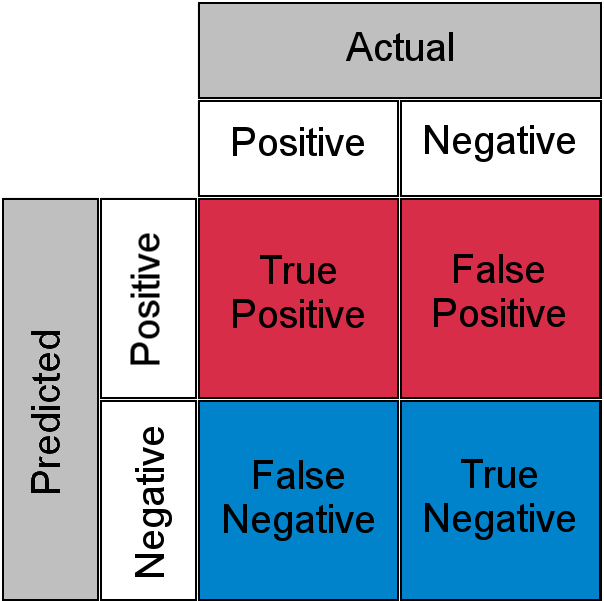
\includegraphics[width=8cm]{\imagesPath/actual_prediction_matrix.png}
    \caption{Actual prediction matrix. From \cite{}}
\end{figure}

Accuracy 
\begin{equation*}
    \frac{TP+TN}{TP+TN+TF+FN}
\end{equation*}

Precision 
\begin{equation*}
    \frac{TP}{TP+FP}
\end{equation*}

\newpage
\section{Linear Regression as Machine Learning}
\textbf{Properties}
\begin{itemize}
    \item Supervised learning algorithm
    \item Numerical variables 
    \item Regression problem
\end{itemize}
\begin{figure}[!h]
    \centering
    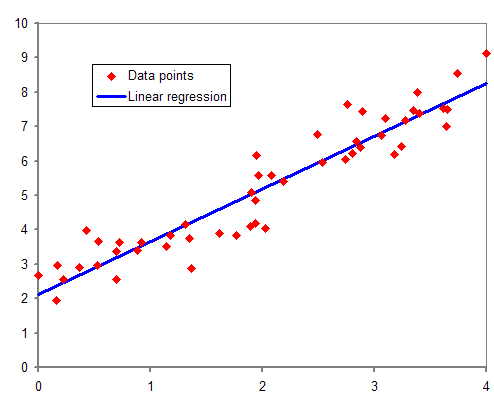
\includegraphics[width=8cm]{\imagesPath/linear_regression.png}
    \caption{Linear regressionFrom \cite{}}
\end{figure}
\href{https://www.youtube.com/watch?v=nk2CQITm_eo}{Explenation}


With the linear hypothesis
\begin{equation*}
    h_{\theta_0,\theta_1(x)} = \theta_0 + \theta_1 x
\end{equation*}
we want the parameters $\theta_0$ and $\theta_1$ to give us as small of a error as possible

the error is calculated with \textbf{Cost function} 
\begin{equation*}
    J(\theta_0,\theta_1) = \frac{1}{2m}\sum_{i=1}^{m}(h_{\theta_0,\theta_1}(x^i)-y^i)^2
\end{equation*}

Where the goal is to \textbf{minimize} $J(\theta_0,\theta_1)$.

\subsection{gradient descent}
%gradient descent is a bad way of doing linear regression. But is good for more complecated algorithms
%to find the values for linear regression we look at wat gets the minimum the squared error
%epochs

Gradient descent can be used for many thing, not so often use for linear regression.
Essentialy what is dose it take a 360 degree view and look at what is the fastest way
to get down the slope. It will repete one step at a time untill it is at a local minimum.

\begin{equation*}
    \frac{\partial}{\partial\theta_j}J(\theta) = \frac{1}{m}\sum_{i=1}^m \left( h_{\theta}(x^{(i)} -y^{(i)})x_j^{(i)} \right)
\end{equation*}
Note that $x_0=1$


\begin{definitionblock}{Linear Regression with Gradient Descent}
    \begin{equation*}
        \theta_0 \gets \theta_0 - \alpha\frac{1}{m}\sum_{i=1}^{m}(\theta_0 + \theta_1(x^{(i)}) - y^{(i)})
    \end{equation*} 
    \begin{equation*}
        \theta_1 \gets \theta_1 - \alpha\frac{1}{m}\sum_{i=1}^{m}(\theta_0 + \theta_1(x^{(i)}) - y^{(i)}) x^{(i)}
    \end{equation*} 
    where $\alpha$ is how aggressive the change should be and $\frac{\partial}{\partial\theta_j}$
    is the angle at the current point, this tells us were we should go and how big of a step.
\end{definitionblock}
$\gets$ and $:=$ is the same thing

If $J$ is minimized then linear regression \textit{always} converges to a global minimum not just a local minimum.
The value of the global minimum dose not need to be $0$ (a line docent need to have a derivative with is $0$).

\href{https://www.youtube.com/watch?v=ErpIw2ohNMs}{Example}
\href{https://machinelearningmastery.com/linear-regression-tutorial-using-gradient-descent-for-machine-learning/}{Discriptive example}


\section{Probability and Naive Bayes Classification}
\textbf{Properties}
\begin{itemize}
    \item Supervised learning algorithm
    \item Categorical variables 
    \item Classification problem
\end{itemize}

By calculating the probability we can decide witch class it belongs to by seeing witch 
has the biggest probability.

\begin{definitionblock}{Bayes theorem}
    \begin{equation*}
        P(H|E) = \frac{P(H)P(E|H)}{P(E)} = \frac{P(H)P(E|H)}{P(H)P(E|H) + P(\neg H)P(E|\neg H)}
    \end{equation*}
    where $H$ is the hypothesis and $E$ is the evidence. $P(H)$ is called the prior, $P(E|H)$ is called the likelihood
    and $P(H|E)$ is the posterior.

\end{definitionblock}

for several cases one can express as followed:
\begin{equation*}
    P(A|b_1,b_2,...,b_n) = \frac{P(b_1|A)P(b_2|A)...P(b_n|A)P(A)}{P(b_1)P(b_2)...P(b_n)}
\end{equation*}

\begin{figure}[!h]
    \centering
    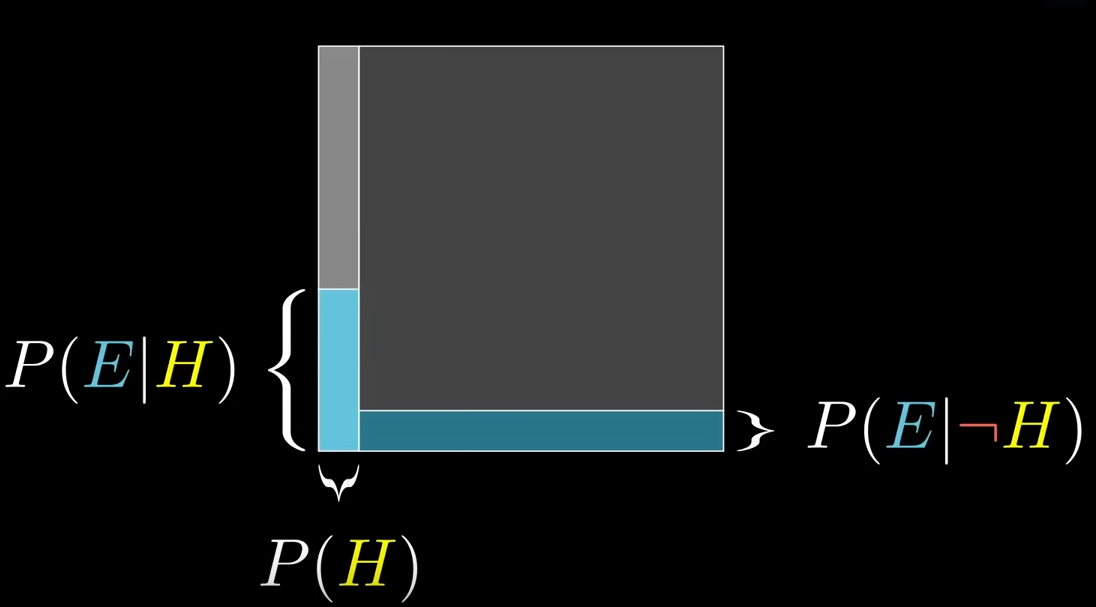
\includegraphics[width=12cm]{\imagesPath/bayes_theorem.png}
    \caption{Bayes Theorem. From \cite{}}
\end{figure}

\begin{itemize}
    \item Experiment: is an outcome of several possible outcomes
    \item Sample space: the set of all possible outcomes
    \item Event: A subset of a sample space
\end{itemize}

%smoothing

\newpage
\section{Logistic Regression}
\textbf{Properties}
\begin{itemize}
    \item Supervised learning algorithm
    \item Numerical and categorical variables 
    \item Classification algorithm
    \item binary classification problems 
\end{itemize}

Linear regression is not good at classification problems, since not all classes can 
be linear separable. Logistic regression is used for classification better than linear regression.
\begin{figure}[!h]
    \centering
    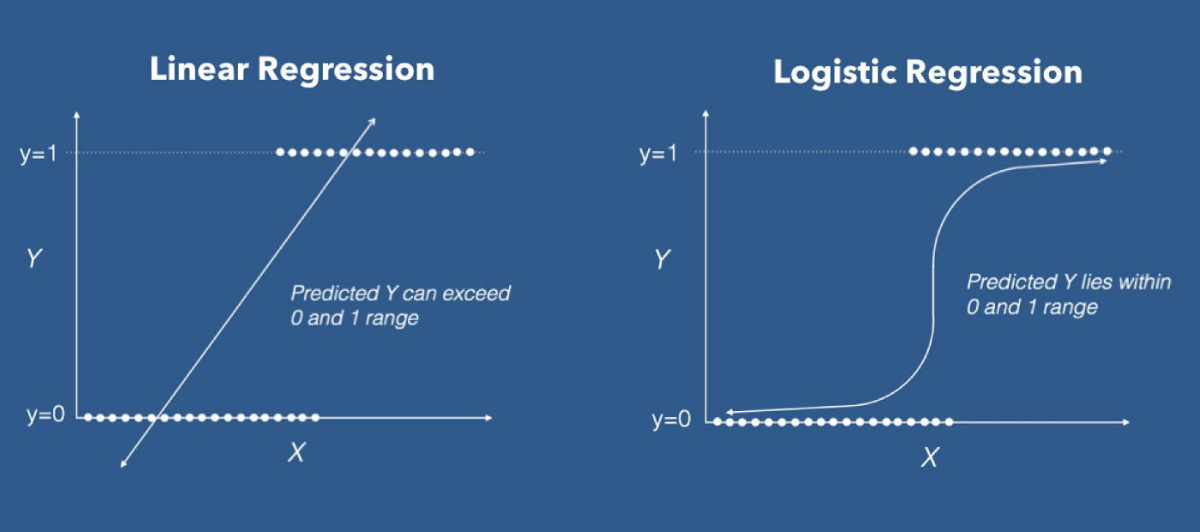
\includegraphics[width=12cm]{\imagesPath/linear_vs_logistic.png}
    \caption{Linear vs logistic regression. From \cite{}}
\end{figure}
\href{https://www.youtube.com/watch?v=-la3q9d7AKQ}{Logistic regression explanation}

The prediction will be for value between $0$ and $1$ so it is best 
for binary classifications. Sigmoid function is the same as logistic function.
\begin{equation*}
    0 \leq h_{\theta}(x) \leq 1
\end{equation*}
\begin{align*}
    h_{\theta}(x) &= g(\theta^T x) \\
    g(z) &= \frac{1}{1+e^{-z}} \\
    &\Rightarrow h_{\theta}(x) = \frac{1}{1+e^{-\theta^T x}} \\
\end{align*}

%Can you use Logistic regression for other classification problems then binary?
%We want to get the probability that it is less then 0.5 for 0 and 1 for the oposite.

%We can have multiple many diffrent times of incerkeld areas since we can have multiple 
%degrees.

\begin{equation*}
    h_{\theta} = g(\theta_0 + \theta_1 x_1 + \theta_2 x_2 + \theta_3 x_1^2 + \theta_4 x_2^2 + \ldots)
\end{equation*}

\subsection{Cost function}
\begin{align*}
    J(\theta) &= \frac{1}{m}\sum_{i=1}^m Cost(h_{\theta}x^{(i)},y^{(i)}) \\
    &= -\frac{1}{m}\left[\sum_{i=1}^m y^{(i)}\log{h_{\theta}(x^{(i)}) + (1-y^{(i)})\log(1-h_{\theta}(x^{(i)}))}\right] \\
\end{align*}

\subsection{Gradient dissent}
\begin{equation*}
    \theta_j := \theta_j -\alpha\sum_{i=1}^m (h_{\theta}(x^{(i)}) - y^{(i)})x_j^{(i)})
\end{equation*}

\begin{equation*}
    J(\theta, x, y) = \frac{1}{2m}\sum_{i=1}^m\left( \sigma\left( \theta^Tx^{(i)} -y^{(i)} \right) \right)^2
\end{equation*}

Multiclass classification problem.
We run classification problem for each class we do logistic regression for 
the class and not class. So if we have tree classes we would have to do tree 
logistic regression hypothesis. Then we can combine them to create a single hypothesis


\subsubsection{Cost function with regularized}
Underfitting is when we use to low of degree of polynomial for the classification.
Overfitting is when the model is to fitted and specific training and therefore preforms badly 
on real data, i.e. to large degree.

We can manually look at the data set and select certain feature.
We can also use a model to automatically do this with regularization.

If we set $\lambda$ to a large number the parameter will automatically be small and 
therefore higher degrees will not effect the output as much.
The legalization parameter $\lambda$ can automatically be determine \newline
\url{https://www.youtube.com/watch?v=IXPgm1e0IOo}

\begin{equation*}
    J(\theta) := \frac{1}{m}\left[\sum_{i=1}^m (h_{\theta}(x^{(i)}) - y^{(i)})^2 + \lambda\sum_{j=1}^n \theta_j^2\right]
\end{equation*}

\subsubsection{Gradient descent with regularization}
\begin{align*}
    \theta_j := \theta_j\left(1-\alpha\frac{\lambda}{m}\right) - \alpha\frac{1}{m}\sum_{i=1}^m \left(h_{\theta}(x^{(i)}) - y^{(i)})x_j^{(i)}\right)
\end{align*}

%\subsubsection{Normal equation}
%\begin{equation*}
%    \theta = 
%    \left( X^T X + \lambda 
%        \begin{bmatrix}
%            0 &   &   &  & \\
%              & 1 &   &  & \\
%              &   & 1 &  & \\
%              &   &   & \ddots & \\
%              &   &   &  & 1 \\
%        \end{bmatrix}
%    \right)^{-1} X^T y
%\end{equation*}


\newpage
\section{Support Vector Machines}
\textbf{Properties}
\begin{itemize}
    \item Supervised learning algorithm
    \item Numerical variables 
    \item classification and regression problems
\end{itemize}
\href{https://www.youtube.com/watch?v=efR1C6CvhmE}{SVM explained}

Support Vector machines are models where tho goal is to find a hyperplane (the line for the two ) with a 
margin either side that maximizes the space between the two clusters.
The labels defining what is in the cluster and not is changed to $-1$ and $1$.

We want to find weights $\bar{w} \in \mathbb{R}^d$ and a constant $b$ such that
\begin{equation*}
    \begin{cases}
        \bar{w} \cdot \bar{x} -b \geq 1 & \text{ if } y=1 \\
        \bar{w} \cdot \bar{x} -b \leq 1 & \text{ if } y=-1
    \end{cases}
\end{equation*}


\begin{figure}[!h]
    \centering
    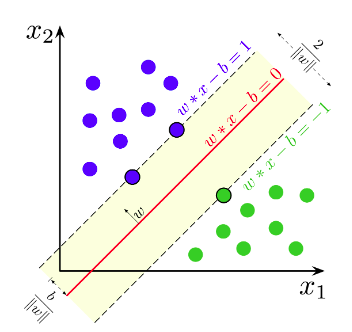
\includegraphics[width=12cm]{\imagesPath/svm_margins_in_2_dim.png}
    \caption{Bayes Theorem. From \cite{}}
\end{figure}


Since the vectors are octagonal to each other the product is 0
\begin{equation*}
    \bar{w}\cdot\bar{x} = 0
\end{equation*}

If we want the vector $\bar{w}$ to be normal to the hyperplane
\begin{align*}
    &\bar{w}\cdot\bar{x} = b \\
    \Rightarrow &\bar{w}\cdot\bar{x} - b = 0
\end{align*}

Hence the two points are $\bar{x}_1$ where $\bar{w}\cdot\bar{x}_1 -b = -1$ and 
$\bar{x}_2$ where $\bar{w}\cdot\bar{x}_2 -b = 1$

%TODO: Dont understand this
Maximisning the distance between the two hyperplanes $\bar{w}x-b=1$ and $\bar{w}x-b=-1$
we want to maximize $t=\frac{2}{||\bar{w}||}$ so we minimize $\frac{1}{2}||\bar{w}||$

\subsection{Quadratic programming}
Graidient descent will not work for all cases if there are a lot of quadratic terms but 
the problem is convex then we can use quadratic programming.

\subsection{Slack Variables}
when there is overlap Quadratic programming will not work

\subsection{kernel trick}
We can compute the inner product in the high-dimensional space by
using a function on the lower dimensional vectors,
i.e. The kernel trick is a way to lower the demission to avoid componential expenses

\subsection{Gaussian Kernels}
\begin{figure}
     \centering
     \begin{subfigure}[b]{0.4\textwidth}
         \centering
         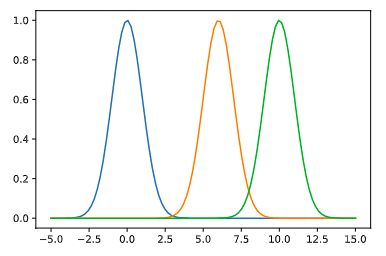
\includegraphics[width=\textwidth]{\imagesPath/gaussian_kernels_1.png}
     \end{subfigure}
     \hfill
     \begin{subfigure}[b]{0.4\textwidth}
         \centering
         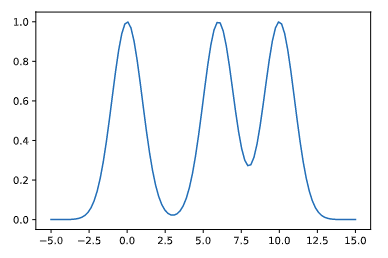
\includegraphics[width=\textwidth]{\imagesPath/gaussian_kernels_2.png}
     \end{subfigure}
        \caption{Gaussian Kernels. From \cite{}}
\end{figure}


\section{Some feature engineering and Cross validation}
\begin{itemize}
    \item Model Bias \newline
    A model is baiased if the error/loss/cost function is high on the training data. It makes bad perdition on the training data.
    \item Model Variance \newline
    A model has high variance if the error/loss/cost function is high on the test data compared with the training data. 
\end{itemize}

Bias variance trade off
\begin{figure}[!h]
    \centering
    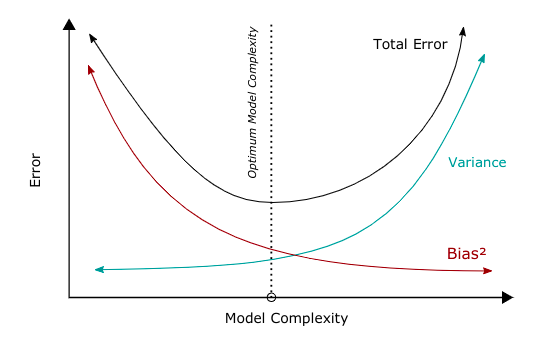
\includegraphics[width=12cm]{\imagesPath/bias_variance_trade_off.png}
    \caption{Bias variance trade off. From \cite{}}
\end{figure}

%TODO
Overfitting vs Bias 

Two Goals
\begin{itemize}
    \item Model Selection: \newline 
    Estimating the performance of different models in order to chose the best one 
    \item Model assessment: \newline 
    Having chosen a final model, estimate its prediction error on new data. 
\end{itemize}

\begin{itemize}
    \item Training \newline
    This is what we use to train our different algorithms. Typical split $50\%$
    \item Validation \newline 
    This is what we use to choose our model we pick the model with the best validation score. Typical split $25\%$
    \item Test \newline 
    This is the data that you keep back until you have picked a model. You use this predict how well you model will do one real data. Typical split $25\%$
\end{itemize}

\subsection{k-fold cross validation}
It is used to evaluate with model is best.

If $k = 5$, then you have $5$ parts $T_1,\ldots,T_5$ you would run $5$ training runs
\begin{itemize}
    \item Train on $T_1, T_2, T_3, T_4$ evaluate on $T_5$.
    \item Train on $T_1, T_2, T_3, T_5$ evaluate on $T_4$.
    \item Train on $T_1, T_2, T_4, T_5$ evaluate on $T_3$.
    \item Train on $T_1, T_3, T_4, T_5$ evaluate on $T_2$.
    \item Train on $T_2, T_3, T_4, T_5$ evaluate on $T_1$.
\end{itemize}
Good values of $k$ are $5$ or $10$. Obviously the larger k is the more time it take to run the experiments.

\textit{Hyper-parameters} \newline
These are parameters to the learning algorithm that do not depend on the data.
They are often continuos values such as the regularization parameter, but not allowance.

\subsection{Estimating Hyper parameters - Grid search}
We make divide our search space of the hyper parameters into a grid (evenly distributed possible values).
Then we go through them all and find the parameters with minimize the error.
\begin{figure}[!h]
    \centering
    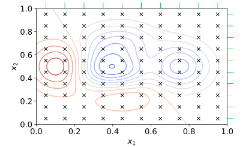
\includegraphics[width=12cm]{\imagesPath/grid_search.png}
    \caption{Grid search. From \cite{}}
\end{figure}
\href{https://www.youtube.com/watch?v=ttE0F7fghfk}{Explanation}


\subsection{One-Hot encoding}
Instead of classifying with natural number like 0, 1, 2 we only 
use 0 and 1. We use 1 for a class and 0 for the other classes.

\subsection{Boosting for feature selection of linear models}
Boosting is a general framework, and it can also be combined with
cross-validation in a technique called bagging (bootstrap aggregating).
The idea is very simple, learn you model one feature at time, at each stage
pick the next feature that gives you optimal performance.
You order the features in order of importance and this gives you models
that are easier to interpret for humans.

Don’t forget to scale your data, so that all dimensions have roughly the
same range

Boosting for linear models advantages
\begin{itemize}
    \item You order the variables in terms of importance
    \item There is the possibility to stop early when the model does not
improve. This is a way of selecting a subset of the features
\end{itemize}

\subsection{Co-variance matrix}
Theremins the covariance between the features in a matrix. 
The larges eigen-value tell us the direction to project in order to 
maximize the variance in that dimension.
\url{https://www.youtube.com/watch?v=152tSYtiQbw}
\url{https://en.wikipedia.org/wiki/Covariance_matrix}


\subsection{Correlation matrix}
How two features are moving with one another. Note that the correlation matrix is diagonally symmetric.
\begin{figure}[!h]
     \centering
     \begin{subfigure}[b]{0.35\textwidth}
         \centering
         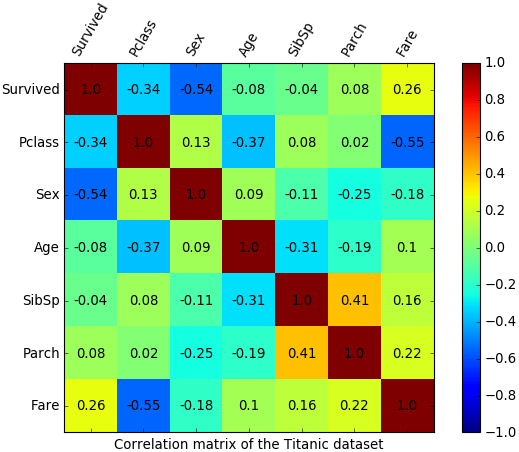
\includegraphics[width=\textwidth]{\imagesPath/corr_matrix.png}
         \caption{Correlation matrix. From \cite{}}
     \end{subfigure}
     \hfill
     \begin{subfigure}[b]{0.55\textwidth}
         \centering
         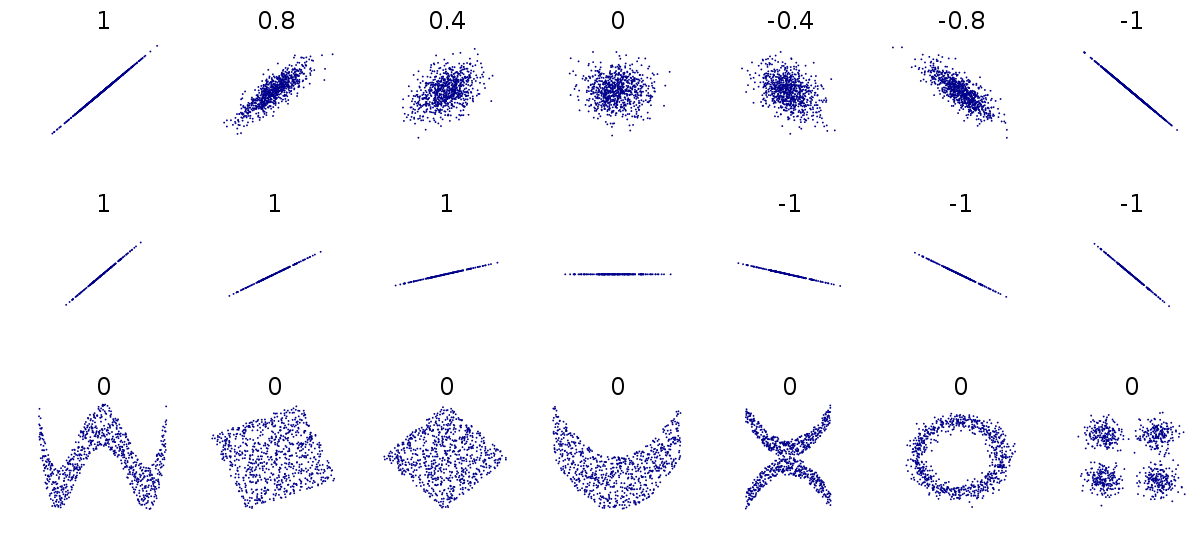
\includegraphics[width=\textwidth]{\imagesPath/correlation.png}
         \caption{Correlation. From \cite{}}
     \end{subfigure}
    \caption{Correlation matrix, the two images are un related}
\end{figure}


\subsection{Heatmap}
This can be done with hierarchical clustering.
\begin{figure}[!h]
    \centering
    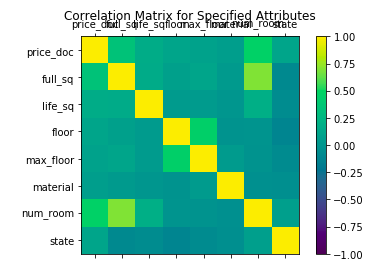
\includegraphics[width=8cm]{\imagesPath/heatmap.png}
    \caption{Heatmap. From \cite{}}
\end{figure}


\section{Clustering and classifiers}
\subsection{k-nearest neighbor classifier}
\textbf{Properties}
\begin{itemize}
    \item Un-supervised learning algorithm
    \item Numerical variables 
\end{itemize}
\begin{figure}[!h]
    \centering
    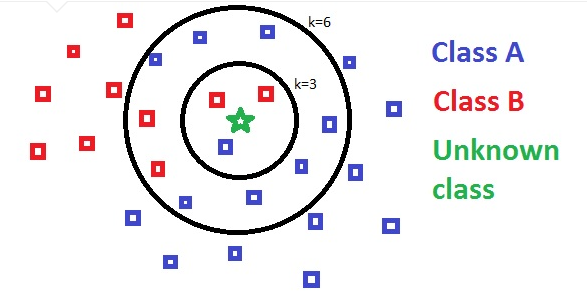
\includegraphics[width=12cm]{\imagesPath/k-nn.png}
    \caption{K-nn. From \cite{}}
\end{figure}


Otherwise known as \textit{k-NN}
\begin{itemize}
    \item Very simple classifier
    \item Memory based, no model is learned you just have to remember the
training data
    \item To classify a point, look at the k -closest points look at their classes
and take a vote
    \item No need to do One-vs-Rest or One-vs-One.
\end{itemize}

Problems with k-NN
\begin{itemize}
    \item As the size of the data set grows, and the more dimensions of the
    input data the computational complexity explodes. This is sometimes
    referred to as the curse of dimensionality
    \item With reasonable clever data structures and algorithms you can speed
things up
\end{itemize}


\subsection{Hierarchical clustering}
\textbf{Properties}
\begin{itemize}
    \item Un-supervised learning algorithm
    \item Numerical and categorical variables 
\end{itemize}

\href{https://www.youtube.com/watch?v=7xHsRkOdVwo}{Hierarchical clustering}

Basic idea:
\begin{itemize}
    \item Start with the same number of clusters as you have data points
    \item At each stage cluster together close together cluster 
    \item Stop when you have enough clusters or everything is clustered together.
\end{itemize}

\begin{figure}[!h]
    \centering
    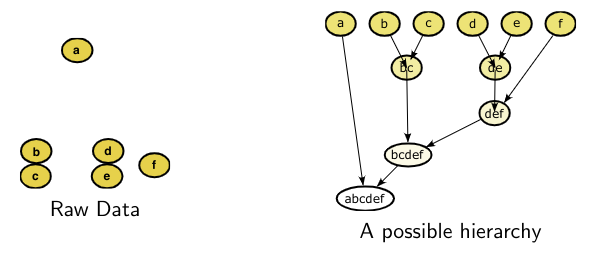
\includegraphics[width=12cm]{\imagesPath/hierarchical_clustering.png}
    \caption{hierarchical clustering. From \cite{}}
\end{figure}

\subsubsection{Linkage Criteria}
The act where a point is associated with a specific class.
\begin{itemize}
    \item Maximum or complete linkage clustering:
    $max\{ d(a,b): a\in A, b\in B\}$
    \item Minimum of single-linkage clustering:
    $min\{ d(a,b): a\in A, b\in B\}$
\end{itemize}

\subsection{K-Means}
\textbf{Properties}
\begin{itemize}
    \item Un-supervised learning algorithm
    \item Numerical variables 
\end{itemize}
\begin{figure}[!h]
    \centering
    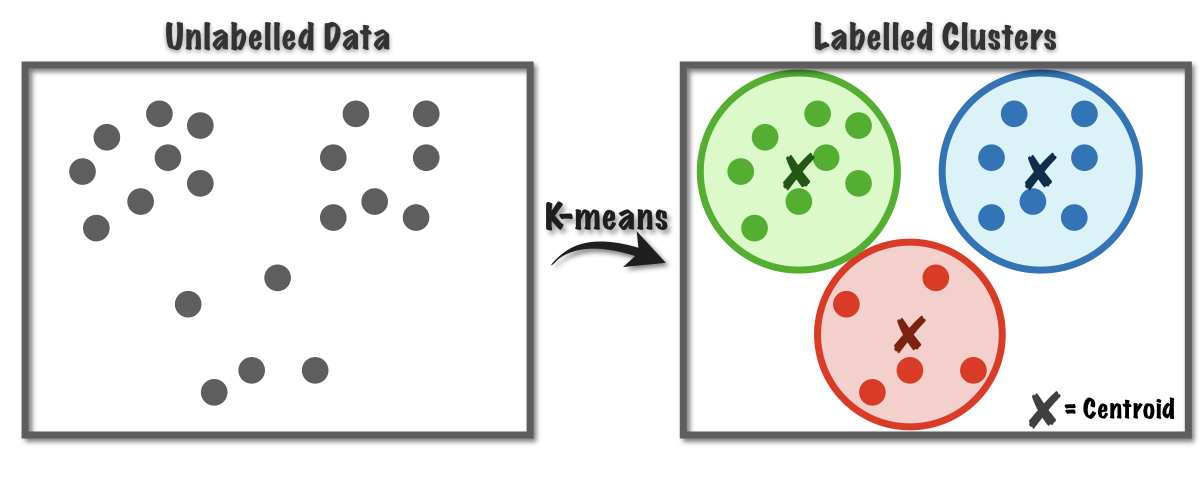
\includegraphics[width=12cm]{\imagesPath/k-means.png}
    \caption{K-means. From \cite{}}
\end{figure}

\begin{equation*}
    \mu = \frac{1}{N} \sum_{i=1}^{n} x_i
\end{equation*}

We want to find $k$ centres $\mu_1,\ldots,\mu_k$ that minimizes the spread or max 
distance in each cluster. 

First we randomly select the clusters centroids. Then we associate each 
point to a cluster with we then replace the centroid so it minimizes it.
Then we repeat this step.  

\href{https://www.youtube.com/watch?v=4b5d3muPQmA}{H-Means explained}

\subsection{DBSCAN}
\textbf{Properties}
\begin{itemize}
    \item Un-supervised learning algorithm
    \item Numerical variables 
\end{itemize}


\begin{figure}[!h]
     \centering
     \begin{subfigure}[b]{0.4\textwidth}
         \centering
         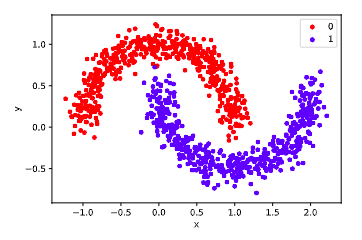
\includegraphics[width=\textwidth]{\imagesPath/DBSCAN_application.png}
         \caption{DBSCAN example. From \cite{}}
     \end{subfigure}
     \hfill
     \begin{subfigure}[b]{0.4\textwidth}
         \centering
         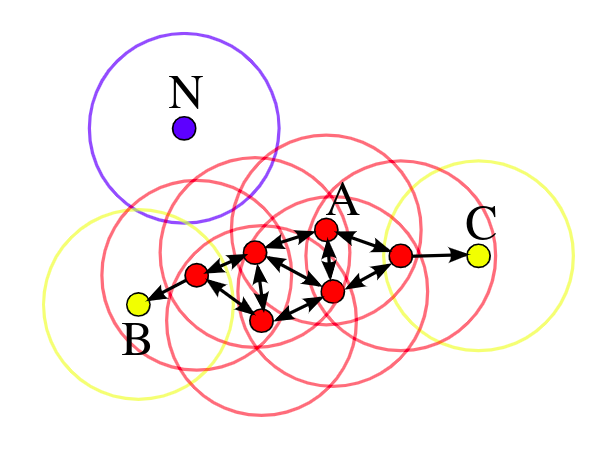
\includegraphics[width=\textwidth]{\imagesPath/DBSCAN_model.png}
         \caption{DBSCAN algorithm. From \cite{}}
     \end{subfigure}
    \caption{DBSCAN}
    \label{fig:DBSCAN}
\end{figure}



\section{Information theory and Decision Theory}
\subsection{Decision Trees}
\textbf{Properties}
\begin{itemize}
    \item Supervised learning algorithm
    \item Categorical variables 
    \item Classification and regression
\end{itemize}

\begin{figure}[!h]
    \centering
    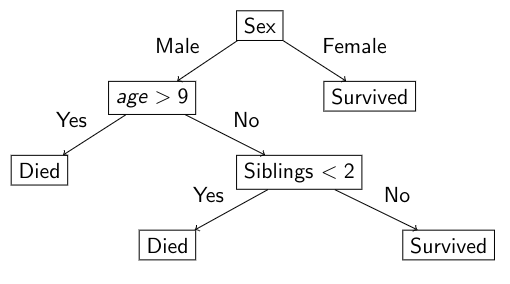
\includegraphics[width=12cm]{\imagesPath/decision_trees.png}
    \caption{Decision Trees. From \cite{}}
\end{figure}
It is NP-hard to find an ordering that gives the smallest tree.
We can get exponential blow up in the size for different orders.
To find the smallest tree we can use information theory.

\subsection{ID3 algorithm}
\begin{enumerate}
    \item Take a feature (with the most entropy) and place it as the root node where the branches true or false or similar (dependent on entropy). Then remove the feature from the feature list.
    \item Then take the new most entropy feature and place it as a node under the parent. Then remove that. 
    \item Then lastly we come to the conclusion (ex diabetes or not diabetes).
\end{enumerate}
\href{https://www.youtube.com/watch?v=aLsReomQ7AA}{ID3 explained}

\subsection{Measuring Information}
\textit{Information theory} is the scientific study of the quantification, 
storage, and communication of digital information.

\textit{Entropy}: a measurement of how spread out the data points are. High entropy means 
that the datapoints ave evenly spread out and 0 means there are not.
\begin{equation*}
    H(X) = -\sum_{i=1}^{n} p_i\log_2(p_i) = \sum_{i=1}^{n} p_i\log_2\left(\frac{1}{p_i}\right)
\end{equation*}

Properies of H and I
Given an event that occurs with probablility $p$ we want a $I(p)$ that measures the 
information of that event. We want $I$ to have certain properties
\begin{itemize}
    \item $I(p)$ is monotonically decreasing in $p$. The higher the probability of the 
    event, the less information.
    \item $I(p) \geq 0$
    \item $I(1) = 0$. An even with probability $1$ has no information.
    \item if $p$ and $q$ are independent events then we want $I(pq) = I(p) + I(p)$
\end{itemize}
Given these properties the only mathematically sensible choice is 
\begin{equation*}
    I(p) = \log\left(\frac{1}{p}\right) = -\log(p)
\end{equation*}

\begin{exampleblock}{Example: Unfair coin with probability $p$}
   \begin{equation*}
       H(p, 1-p) = -p\log p -(1-p)\log(1-p)
   \end{equation*} 

   If you plot the graph it will look something like figure 
\end{exampleblock}
\begin{figure}[!h]
    \centering
    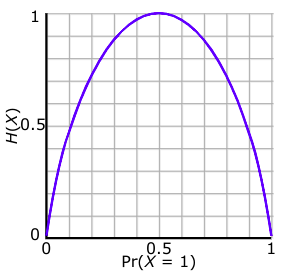
\includegraphics[width=6cm]{\imagesPath/unfair_coin.png}
    \caption{Decision Trees. From \cite{}}
\end{figure}

\textit{Conditional entropy}
\begin{equation*}
    H(X|Y=a) = -\sum_{x\in X}P(x|Y=a)\log_2 P(x|Y=a)
\end{equation*}
where $P(X|Y) = \frac{P(X,Y)}{P(X)}$

\textit{Information Gain}
\begin{figure}[!h]
    \centering
    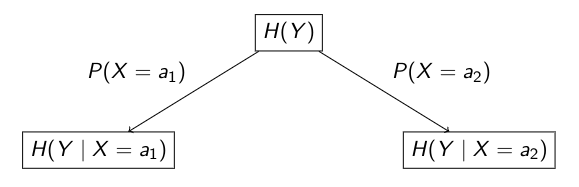
\includegraphics[width=10cm]{\imagesPath/information_gain.png}
    \caption{Decision Trees. From \cite{}}
\end{figure}

\begin{equation*}
    H(Y) - \left( \underbrace{P(X=a_1)H(Y|X=a_1) + P(X=a_2)H(Y|X=a_2)}_{\text{average information when split}} \right)
\end{equation*}

\textbf{ID3 algorithm} the algorithm to construct a tree using information
theory.
\begin{itemize}
    \item ID3 is heuristic, i.e. practical solution but not optimal result, since we use information there to make it easier to solve.
    \item ID3 will not construct the smallest tree.
\end{itemize}

\begin{figure}[!h]
    \centering
    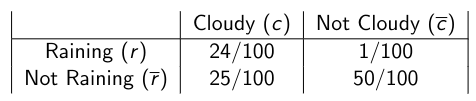
\includegraphics[width=10cm]{\imagesPath/example_conditional_entropy.png}
    \caption{Example Conditional Entropy. From \cite{}}
    \label{fig:example_conditional_entropy}
\end{figure}
\begin{exampleblock}{Example: Conditional entropy}
    Se figure \ref{fig:example_conditional_entropy}
    The amount of days it is raining ($24+1=25$)
    \begin{itemize}
        \item $P(c|r) = 24/25$
        \item $P(\bar{c}|r) = 1/25$ 
    \end{itemize}
    
    \begin{equation*}
        H(Y|X=r) = -\underbrace{\frac{24}{25}\log_2\frac{24}{25}}_{\text{Cloudy}} - \overbrace{\frac{1}{25}\log_2\frac{1}{25}}^{\text{NotCloudy}} \approx 0.24
    \end{equation*}
\end{exampleblock}

Advantages of Decision trees
\begin{itemize}
    \item Easy to understand what the algorithm has learned 
    \item Can learn very non-linear boundaries
    \item Does not require that much processing
    \item Not many parameters to tune 
\end{itemize}

Disadvantages of Decision trees
\begin{itemize}
    \item Prone to overfilling 
    \item Small changes in the data can mean that you learn very different trees.
    \item Computationally more expressive than other methods
\end{itemize}

\section{Principle component analysis (PCA)}
Is dimensionality reduction method, i.e. reducing the number of dimension of a training set.
We try to compress the data, i.e. remove the redundant data.
\begin{figure}[!h]
    \centering
    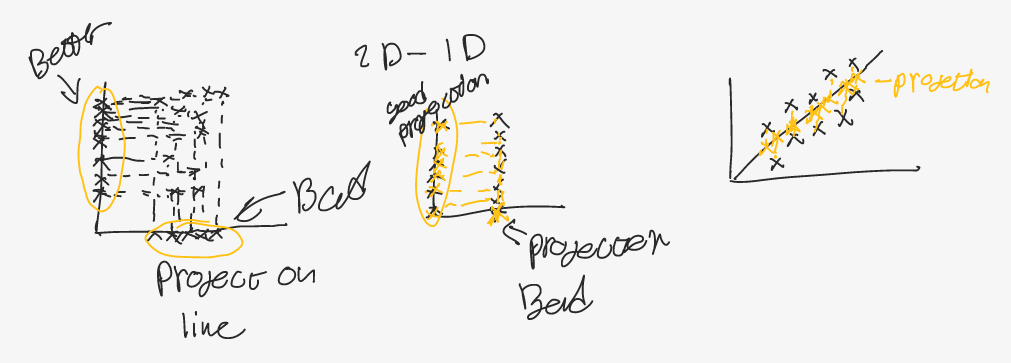
\includegraphics[width=10cm]{\imagesPath/pca_demo.png}
    \caption{Example Conditional Entropy}
    \label{fig:pca_demo}
\end{figure}

covariance matrix is 
\begin{align*}
   B &= X - \bar{X}  \\
   C &= B^TB
\end{align*}
where $X$ is the data matrix.

\begin{equation*}
    C\omega = \lambda\omega
\end{equation*}
Where $C$ is Covariance matrix, $\lambda$ is the eigenvalue and $\omega$ is the eigenvector
\href{https://www.youtube.com/watch?v=fkf4IBRSeEc}{PCA discription}

The principle components 
\begin{equation*}
    T = B\omega
\end{equation*}

We then \textbf{reduse the dimension} by desigding on how many principle component we want
this is done by taking the standard diviation to including $x\%$ of the data.


\subsection{Covariance Matrix}
Is a diagonaly symetric matrix of the covariance between two elements in the random vector.

The eigenvectors of the covariance matrix describes the direction of the line where the
data points are maped to.
\url{https://wiki.pathmind.com/eigenvector}


\url{https://www.youtube.com/watch?v=pmG4K79DUoI}
\url{https://www.youtube.com/watch?v=rng04VJxUt4}

When the eigenvalues are relativly small we can remove those vectors since the do 
not contrebute much of the eigenvalue is in significant.


%\section{For the exam}
%To be added 
%\begin{itemize}
    %\item (l4, s28) Cross Entropy Cost?
    %\item What is smoothening? It is a preprosessing technique where the data were you average out the data 
    %\item Overfitting vs Bias? Bias can refer to multiple things one of witch is bias data like with volvos in sweden. Or with to much training data, in this case it could couse overfitting.
    %\item \url{https://www.sciencedirect.com/topics/computer-science/logistic-regression}
%\end{itemize}
%
%questions missing from exam 
%\begin{itemize}
    %\item what is gradient descent how does it work?
    %\item How does SVM work 
    %\item bias variance
%\end{itemize}